\documentclass[a4paper,10pt]{jsarticle}

% 数式
\usepackage{amsmath,amsfonts}
\usepackage{bm}
% 画像
\usepackage[dvipdfmx]{graphicx}
\usepackage{here}

\usepackage{listingsutf8,jlisting} %日本語のコメントアウトをする場合jlistingが必要
%ここからソースコードの表示に関する設定
\lstset{
  basicstyle={\ttfamily},
  identifierstyle={\small},
  commentstyle={\smallitshape},
  keywordstyle={\small\bfseries},
  ndkeywordstyle={\small},
  stringstyle={\small\ttfamily},
  frame={tb},
  breaklines=true,
  columns=[l]{fullflexible},
  numbers=left,
  xrightmargin=0zw,
  xleftmargin=3zw,
  numberstyle={\scriptsize},
  stepnumber=1,
  numbersep=1zw,
  lineskip=-0.5ex
}

\begin{document}

\title{第7回演習課題}
\author{坪井正太郎(101830245)}
\date{\today}
\maketitle
\section{3番地コード}
\begin{lstlisting}[caption={3番地コード},label={3番地コード}]
    i=1
    j=1
    k=0
l1: t=k<100
    if not t goto l2
    n=j<20
    if not n goto l3
    j=i
    k=k+1
    goto l4
l3: j=k
    k=k+2
l4: goto l1
l2: k=k+3
\end{lstlisting}

\section{フローグラフ、支配木}
\begin{figure}[H]
  \centering
  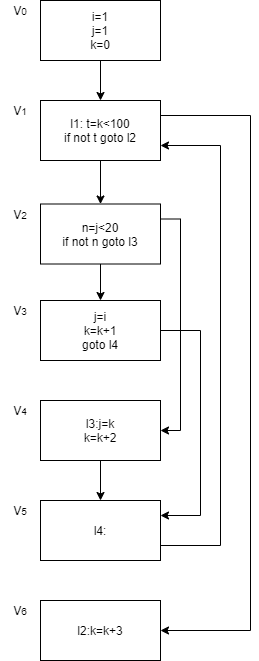
\includegraphics[width=7cm]{01.drawio.png}
\end{figure}
\begin{figure}[H]
  \centering
  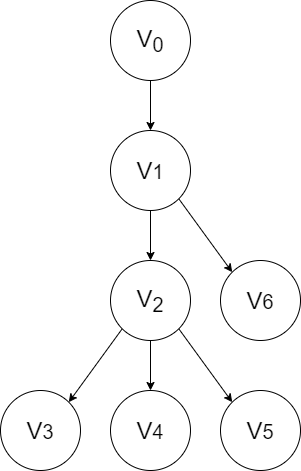
\includegraphics[width=7cm]{02.drawio.png}
\end{figure}

\section{頂点集合}
iの定義 $S_0=\{V_0\}$

jの定義 $S^\prime_0=\{V_0,V_3,V_4\}$

jの定義 $S^{\prime\prime}_0=\{V_0,V_3,V_4,V_6\}$

iの頂点集合 $DE^+(S_0)=\emptyset$

jの頂点集合 $DE^+(S^\prime_0)=\{V_1,V_5\}$

jの頂点集合 $DE^+(S^{\prime\prime}_0)=\{V_1,V_5\}$

\section{SSAコード}
\begin{lstlisting}[caption={SSA形式},label={SSA形式}]
  i1=1
  j1=1
  k1=0
l1: j2=phi(j1,j5)
    k2=phi(k1,k5)
    t=k2<100
    if not t goto l2
    n=j2<20
    if not n goto l3
    j3=i1
    k3=k2+1
    goto l4
l3: j4=k2
    k4=k2+2
l4: j5=phi(j3,j4)
    k5=phi(k3,k4)
    goto l1
l2: k6=k2+3
\end{lstlisting}

\section{$\phi$関数の除去}
\begin{lstlisting}[caption={除去後},label={除去後}]
    i1=1
    j1=1
    k1=0
    j2=j1
    k2=k1
l1: t=k2<100
    if not t goto l2
    n=j2<20
    if not n goto l3
    j3=i1
    k3=k2+1
    j5=j3
    k5=k3
    goto l4
l3: j4=k2
    k4=k2+2
    j5=j4
    k5=k4
l4: j2=j5
    k2=k5
    goto l1
l2: k6=k2+3
\end{lstlisting}

\end{document}
